\documentclass[letterpaper]{article}
\usepackage{aaai23}
\usepackage{times}
\usepackage{helvet}
\usepackage{courier}
\usepackage[hyphens]{url}
\usepackage{graphicx}
\urlstyle{rm} 
\def\UrlFont{\rm}  
\usepackage{natbib}
\usepackage{caption}
\usepackage{tikz}
\frenchspacing  
\setlength{\pdfpagewidth}{8.5in}  
\setlength{\pdfpageheight}{11in}  

\title{Image Classification with Neural Networks: An Experimental Study}
\author{Robert Nasuti\\
University of Colorado at Colorado Springs\\
rnasuti@uccs.edu}

\begin{document}

\maketitle

\begin{abstract}
This paper presents an exploration into the domain of image classification using artificial neural networks. We investigate the performance of custom CNN architectures and compare them with widely-recognized networks like VGG16 and ResNet50 on popular datasets including MNIST, CIFAR-10, and Tiny Imagenet.
\end{abstract}

\section{Introduction}
Image classification, a fundamental task in the domain of computer vision, involves categorizing an input image into one of several predefined classes. With the advent of deep learning, convolutional neural networks (CNNs) have been at the forefront of achieving remarkable performance on this task. In this study, we explore the capabilities of custom CNN architectures and benchmark them against renowned models on three datasets: MNIST, CIFAR-10, and Tiny Imagenet.

\section{Approach}

\subsection{Datasets}

\subsubsection{MNIST}
MNIST is a large database of handwritten digits. It contains 60,000 training images and 10,000 testing images, each of size 28x28 pixels.

\subsubsection{CIFAR-10}
CIFAR-10 consists of 60,000 32x32 color images in 10 classes, with 6,000 images per class. There are 50,000 training images and 10,000 test images.

\subsubsection{Tiny Imagenet}
Tiny Imagenet is a subset of the larger ImageNet dataset, containing 200 classes. Each class has 500 training images, 50 validation images, and 50 test images.

\begin{table}[h]
    \centering
    \resizebox{\columnwidth}{!}{%
    \begin{tabular}{|l|l|}
    \hline
    \textbf{Dataset \& Model} & \textbf{Pre-processing} \\
    \hline
    1-layer-cnn MNIST & Reshape to (60000, 28, 28, 1), Normalize \\
    \hline
    1-layer-cnn CIFAR-10 & Normalize \\
    \hline
    1-layer-cnn \& LeNet-5 Tiny Imagenet & Resize to 64x64, Batch size: 128 \\
    \hline
    VGG16 MNIST & Resize to (32, 32), Normalize \\
    \hline
    VGG16 CIFAR-10 & Normalize \\
    \hline
    VGG16 Tiny Imagenet & Resize to 64x64, Batch size: 64 \\
    \hline
    ResNet50 MNIST & Resize to (32, 32), Normalize \\
    \hline
    ResNet50 CIFAR-10 & Normalize \\
    \hline
    ResNet50 Tiny Imagenet & Resize to 64x64, Batch size: 64 \\
    \hline
    \end{tabular}%
    }
    \caption{Pre-processing steps for each dataset and model.}
    \label{tab:preprocessing}
    \end{table}
    
\subsection{Models}

\subsubsection{1-Layer CNN}
Our custom 1-layer CNN architecture primarily consists of a convolutional layer followed by a dense layer, as illustrated in Figure \ref{fig:1layercnn}.
\begin{figure}
    \centering
    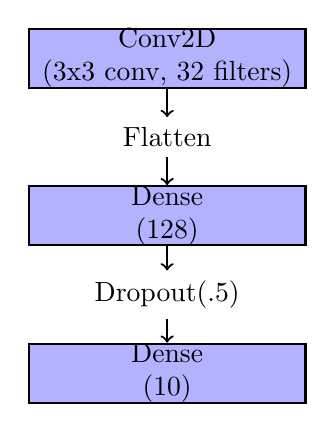
\begin{tikzpicture}[thick, node distance=.5cm]
        \tikzstyle{layer}=[rectangle,draw=black,fill=blue!30,minimum size=20pt,inner sep=0pt,minimum width=100pt, minimum height=20pt, align=center]

        \node[layer] (conv) {Conv2D\\(3x3 conv, 32 filters)};
        \node[below of=conv, node distance=1cm] (flatten) {Flatten};
        \node[layer, below of=flatten, node distance=1cm] (dense1) {Dense\\(128)};
        \node[below of=dense1, node distance=1cm] (dropout) {Dropout(.5)};
        \node[layer, below of=dropout, node distance=1cm] (dense2) {Dense\\(10)};
        
        \draw[->] (conv) -- (flatten);
        \draw[->] (flatten) -- (dense1);
        \draw[->] (dense1) -- (dropout);
        \draw[->] (dropout) -- (dense2);
    \end{tikzpicture}
    \caption{1-Layer CNN architecture.}
    \label{fig:1layercnn}
\end{figure}

\subsubsection{LeNet-5}
Inspired by the classic LeNet-5 architecture, our adapted model is illustrated in Figure \ref{fig:lenet5}.
\begin{figure}
    \centering
    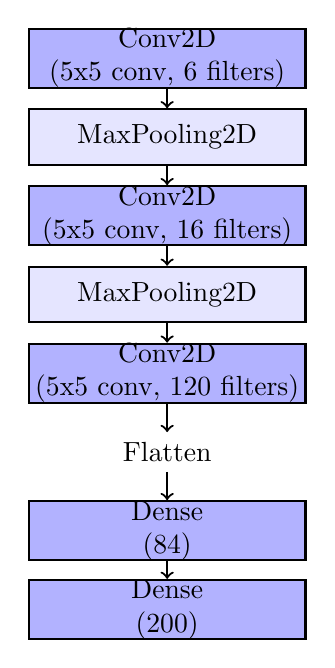
\begin{tikzpicture}[thick, node distance=0.5cm]
        \tikzstyle{layer}=[rectangle,draw=black,fill=blue!30,minimum size=20pt,inner sep=0pt,minimum width=100pt, minimum height=20pt, align=center]
        \tikzstyle{pool}=[rectangle,draw=black,fill=blue!10,minimum size=20pt,inner sep=0pt,minimum width=100pt, minimum height=20pt, align=center]

        \node[layer] (conv1) {Conv2D\\(5x5 conv, 6 filters)};
        \node[pool, below of=conv1, node distance=1cm] (pool1) {MaxPooling2D};
        \node[layer, below of=pool1, node distance=1cm] (conv2) {Conv2D\\(5x5 conv, 16 filters)};
        \node[pool, below of=conv2, node distance=1cm] (pool2) {MaxPooling2D};
        \node[layer, below of=pool2, node distance=1cm] (conv3) {Conv2D\\(5x5 conv, 120 filters)};
        \node[below of=conv3, node distance=1cm] (flatten) {Flatten};
        \node[layer, below of=flatten, node distance=1cm] (dense1) {Dense\\(84)};
        \node[layer, below of=dense1, node distance=1cm] (dense2) {Dense\\(200)};
        
        \draw[->] (conv1) -- (pool1);
        \draw[->] (pool1) -- (conv2);
        \draw[->] (conv2) -- (pool2);
        \draw[->] (pool2) -- (conv3);
        \draw[->] (conv3) -- (flatten);
        \draw[->] (flatten) -- (dense1);
        \draw[->] (dense1) -- (dense2);
    \end{tikzpicture}
    \caption{Customized LeNet-5 architecture.}
    \label{fig:lenet5}
\end{figure}

\subsubsection{VGG16 and ResNet50}
VGG16 and ResNet50 are widely-recognized architectures that have been extensively utilized in various computer vision tasks, especially image classification, due to their robustness and reliability. VGG16 is known for its simplicity, using only 3x3 convolutional layers stacked on top of each other in increasing depth. ResNet50 leverages a deep architecture with skip connections to prevent the loss of information through the network’s depth.

\subsubsection{Modified ResNet50 for Tiny ImageNet}
For the Tiny ImageNet dataset, we utilized a modified version of the ResNet50 model, integrating additional dense and dropout layers to manage the complexity and prevent overfitting. The architecture is illustrated in Figure \ref{fig:modresnet50}.
\begin{figure}
    \centering
    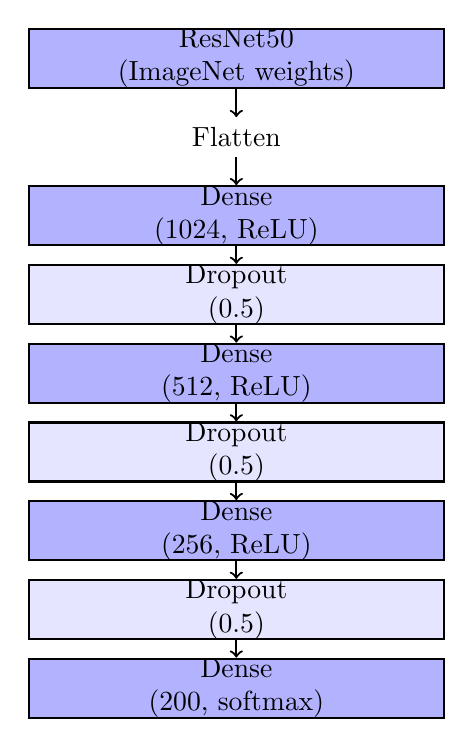
\begin{tikzpicture}[thick, node distance=0.5cm]
        \tikzstyle{layer}=[rectangle,draw=black,fill=blue!30,minimum size=20pt,inner sep=0pt,minimum width=150pt, minimum height=20pt, align=center]
        \tikzstyle{dropout}=[rectangle,draw=black,fill=blue!10,minimum size=20pt,inner sep=0pt,minimum width=150pt, minimum height=20pt, align=center]

        \node[layer] (base) {ResNet50\\(ImageNet weights)};
        \node[below of=base, node distance=1cm] (flatten) {Flatten};
        \node[layer, below of=flatten, node distance=1cm] (dense1) {Dense\\(1024, ReLU)};
        \node[dropout, below of=dense1, node distance=1cm] (dropout1) {Dropout\\(0.5)};
        \node[layer, below of=dropout1, node distance=1cm] (dense2) {Dense\\(512, ReLU)};
        \node[dropout, below of=dense2, node distance=1cm] (dropout2) {Dropout\\(0.5)};
        \node[layer, below of=dropout2, node distance=1cm] (dense3) {Dense\\(256, ReLU)};
        \node[dropout, below of=dense3, node distance=1cm] (dropout3) {Dropout\\(0.5)};
        \node[layer, below of=dropout3, node distance=1cm] (dense4) {Dense\\(200, softmax)};
        
        \draw[->] (base) -- (flatten);
        \draw[->] (flatten) -- (dense1);
        \draw[->] (dense1) -- (dropout1);
        \draw[->] (dropout1) -- (dense2);
        \draw[->] (dense2) -- (dropout2);
        \draw[->] (dropout2) -- (dense3);
        \draw[->] (dense3) -- (dropout3);
        \draw[->] (dropout3) -- (dense4);
    \end{tikzpicture}
    \caption{Modified ResNet50 architecture for Tiny ImageNet.}
    \label{fig:modresnet50}
\end{figure}

\section{Experimental Setup}
In the experiments, we utilized the Adam optimizer and categorical crossentropy as the loss function, which is suitable for the multi-class classification problems presented by our datasets. The models were trained using an Nvidia 4090 GPU, leveraging its computational capability to efficiently train the deep learning models. The operating system used was Ubuntu 22.04 LTS, and models were implemented using Keras with a TensorFlow backend. 

Specifically, the activation function for hidden layers was set to ReLU (Rectified Linear Unit) to introduce non-linearity into the model, while the output layer utilized a softmax activation function to produce a probability distribution over the target classes. To find the optimal batch size and learning rate for each model-dataset combination, several runs were performed with varied parameters, ensuring that model learning was stable and converged efficiently. In most scenarios, convergence was observed after approximately 20 epochs.

The datasets underwent a series of preprocessing steps, which were critical to ensure the consistency of input data and to enhance the training efficiency and model performance. The specific preprocessing steps for each dataset and model are detailed in Table \ref{tab:preprocessing}. 

\section{Results}

In this section, we present the performance of our models on the respective datasets in terms of accuracy. A comprehensive visual comparison of the accuracy achieved by each model on different datasets is provided in Figure \ref{fig:accuracycomparison}.

\textbf{1-Layer CNN:} 
\begin{itemize}
    \item MNIST: 0.9852 maximum accuracy on the validation set.
    \item CIFAR-10: 0.6343 maximum accuracy on the validation set.
    \item Tiny ImageNet: 0.005 maximum accuracy on the validation set.
\end{itemize}

\textbf{LeNet-5:} 
\begin{itemize}
    \item Tiny ImageNet: 0.1737 maximum accuracy on the validation set.
\end{itemize}

\textbf{VGG-16:} 
\begin{itemize}
    \item MNIST: No pre-training, fine-tuned for 20 epochs, maximum accuracy of 0.9941 observed.
    \item CIFAR-10: No pre-training, model failed to learn after 20 epochs, resulting in a maximum accuracy of 0.1 against the validation set and lower on the training set.
    \item Tiny ImageNet: No pre-training, model failed to learn after 20 epochs, maximum accuracy of 0.005 against the validation set and lower on the training set.
    \item CIFAR-10 with ImageNet weights: Froze the base model and fine-tuned for 5 epochs, then unfroze bottom 4 layers and trained for another 20 epochs, achieving a maximum accuracy of 0.7433.
    \item Tiny ImageNet with ImageNet weights: Froze the base model and fine-tuned for 5 epochs, then unfroze bottom 4 layers and trained for another 20 epochs, achieving a maximum accuracy of 0.4229.
\end{itemize}

\textbf{ResNet50:} 
\begin{itemize}
    \item MNIST: Did not freeze any layers, fine-tuned for 20 epochs, achieving a maximum accuracy of 0.9932 against the validation set.
    \item CIFAR-10: Did not freeze any layers, fine-tuned for 20 epochs, achieving a maximum accuracy of 0.8039 against the validation set.
    \item Tiny ImageNet: Did not freeze any layers, fine-tuned for 20 epochs, achieving a maximum accuracy of 0.2729 against the validation set.
\end{itemize}

\begin{figure}
    \centering
    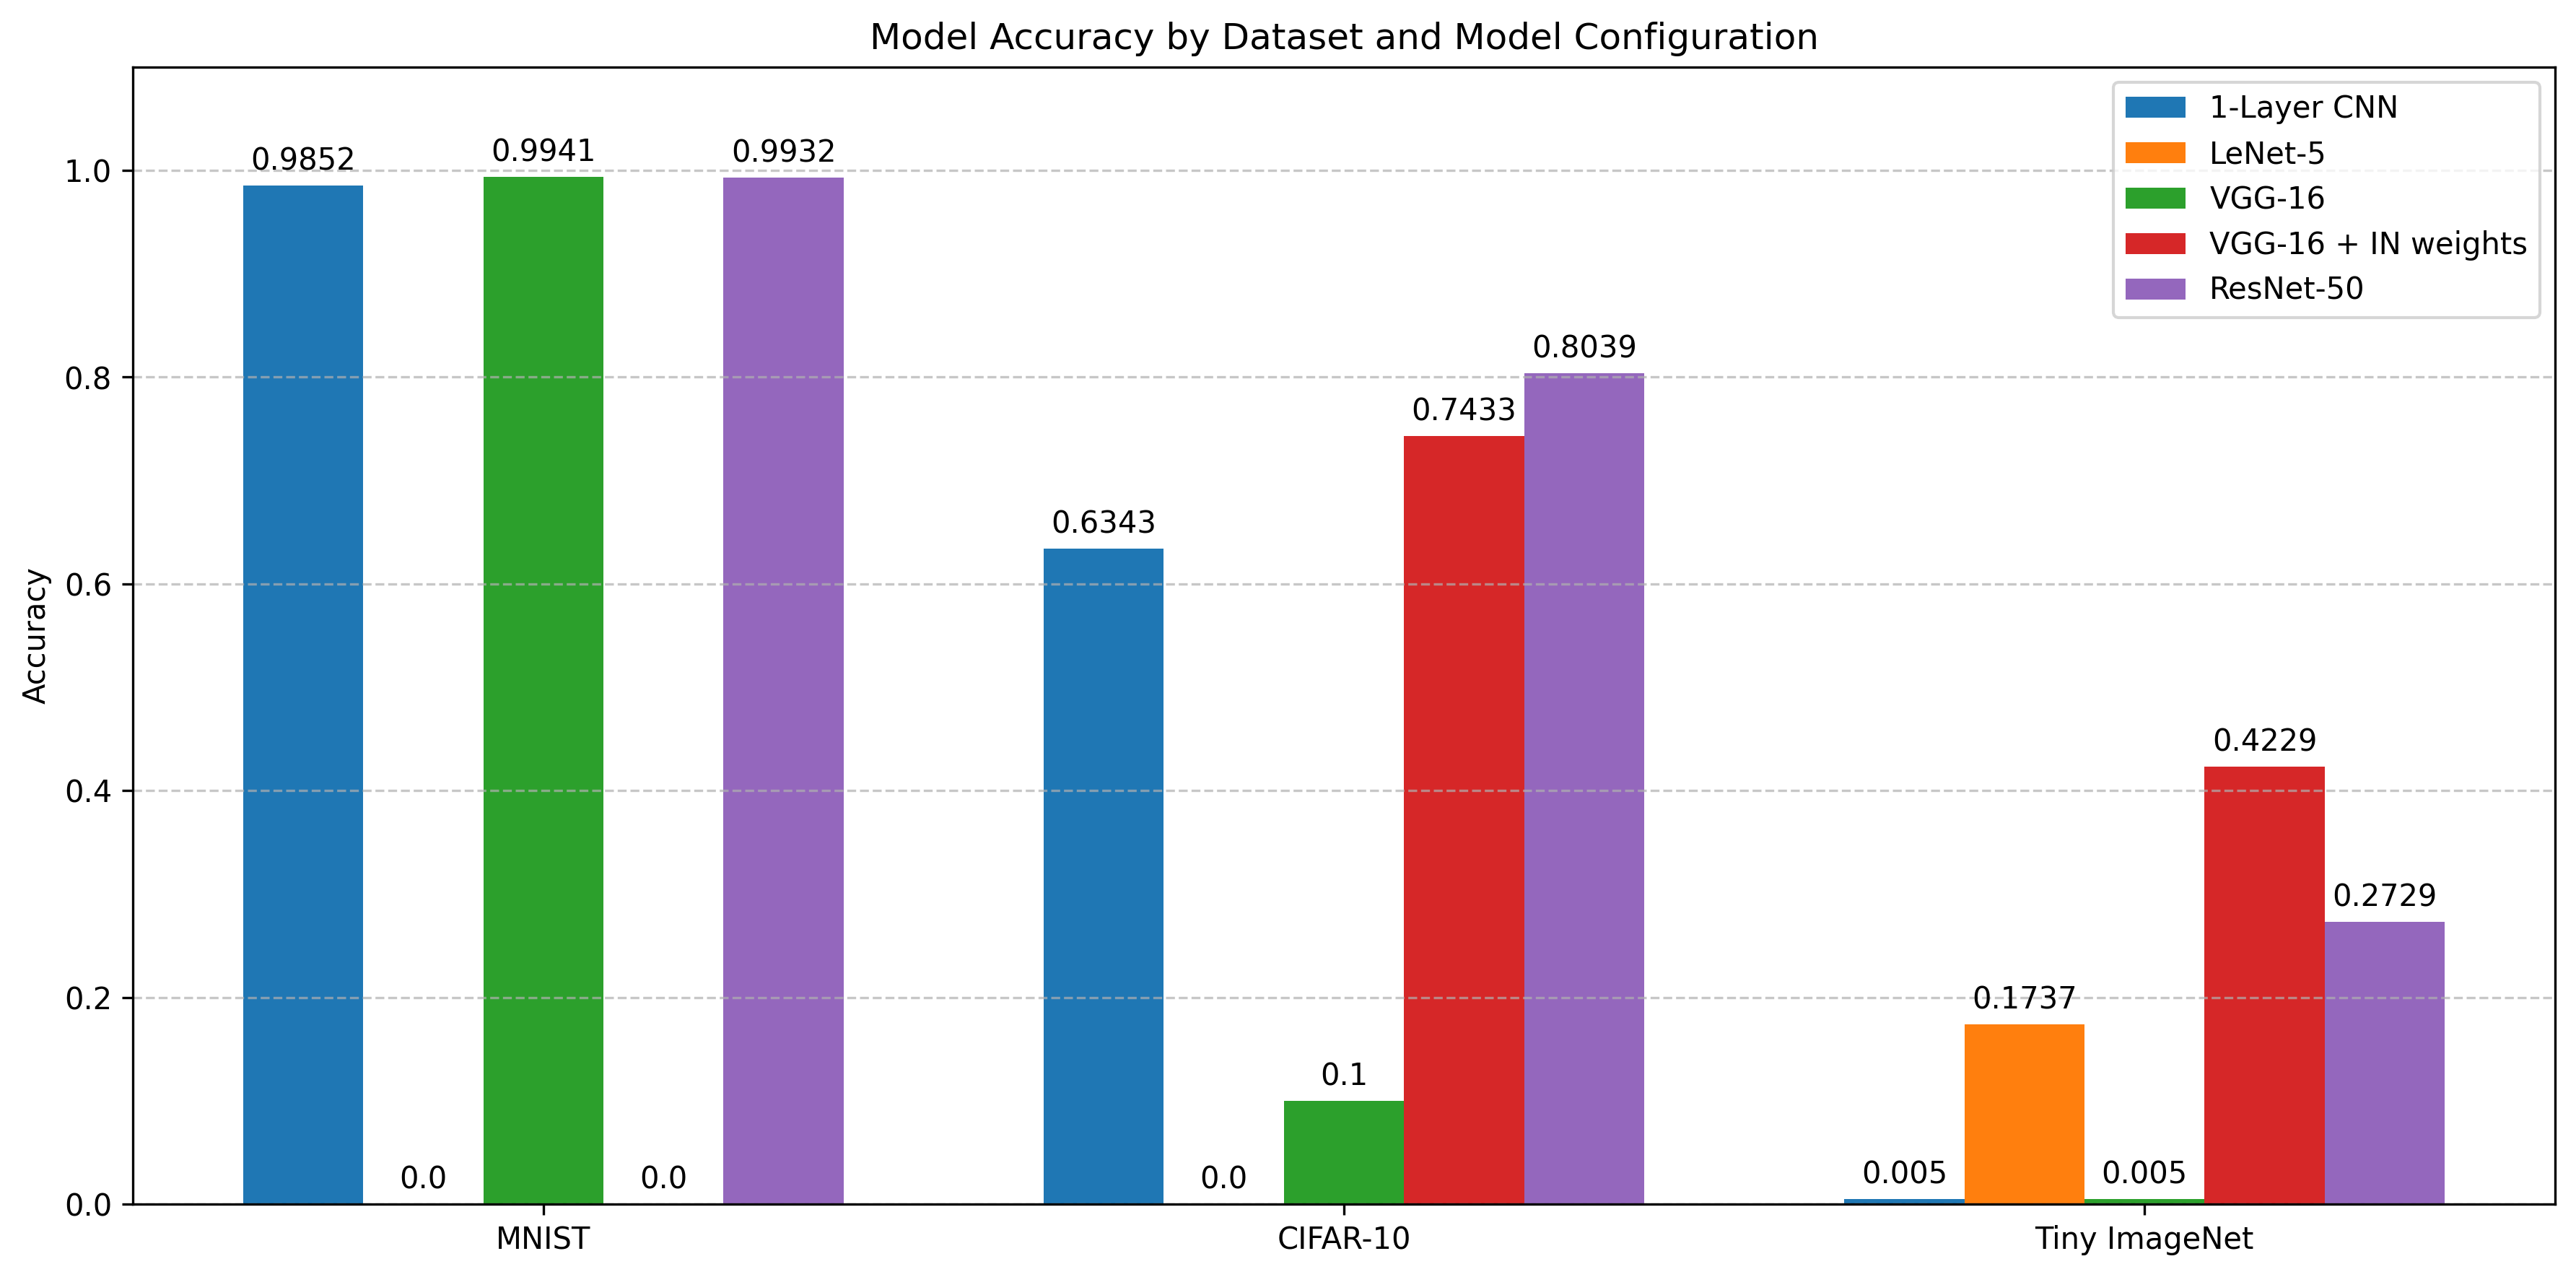
\includegraphics[width=0.8\linewidth]{accuracy_comparison.png}
    \caption{Comparison of classification accuracies across different neural network models and datasets. The models, of increasing complexity, are evaluated on three datasets: MNIST, CIFAR-10, and Tiny ImageNet. Accuracies are depicted as bar heights, and each model's performance on a dataset is represented by a distinct bar, facilitating direct visual comparison. Notably, model performance varies significantly across different datasets. A measurement value of 0.0 signifies that the respective dataset was not utilized for the evaluation of the corresponding model. In such instances, the absence of a recorded accuracy metric should not be misconstrued as a zero-accuracy outcome, but rather as an indication that the model was not subjected to testing against that specific dataset.}
    \label{fig:accuracycomparison}
\end{figure}

\section{Observations}
Building upon the results presented in the previous section, this section aims to provide insights and draw observations from the performance metrics of various models across different datasets.

\begin{itemize}
    \item The 1-layer CNN was sufficient for MNIST but not for Tiny ImageNet, indicating a necessity for deeper architectures for more complex datasets.
    \item The LeNet-5 model performed surprisingly well on Tiny ImageNet, given its relatively simple architecture.
    \item VGG-16 was able to learn MNIST from scratch but struggled with CIFAR-10 and Tiny ImageNet, which was unexpected given the complexity of the network.
    \item Fine-tuning VGG-16 and ResNet-50 on MNIST and CIFAR-10 resulted in early overfitting, followed by a rapid increase in validation performance before plateauing, potentially exhibiting the "Grokking" phenomenon as described in "GROKKING: Generalization Beyond Overfitting on Small Algorithmic Datasets." \cite{power2022grokking}
    \item ResNet-50 demonstrated overfitting when used alone, which is indicated by a disparity in validation and training data performance (see Figure \ref{fig:overfittinggraph}). Introducing dropout layers as a form of regularization mitigated overfitting but resulted in "spiky" validation performance, as can be seen in Figure \ref{fig:spikygraph}, warranting further investigation.
    \item Freezing layers during the training of ResNet-50 seemed to slow or prevent the network from learning. Initially, unfreezing only 4 layers, then 25, and finally all of them was attempted. Unfreezing the entire model yielded the best performance, suggesting that perhaps due to the "skip architecture" of ResNet-50, freezing layers might not be the most effective approach for this particular architecture.
\end{itemize}
\begin{figure}
    \centering
    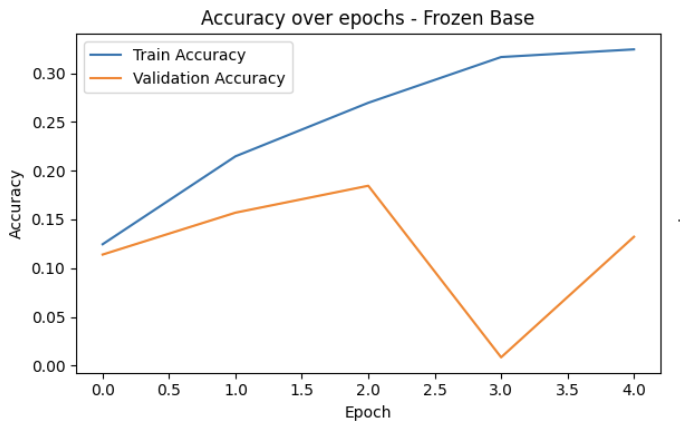
\includegraphics[width=0.8\linewidth]{resnet50_tiny_imagenet_overfitting.png}
    \caption{Training and validation accuracy of ResNet-50 on Tiny ImageNet, illustrating overfitting. The graph demonstrates a growing divergence between training and validation accuracy as epochs progress, indicative of the model memorizing the training data and losing generalization on the validation data.}
    \label{fig:overfittinggraph}
\end{figure}
\begin{figure}
    \centering
    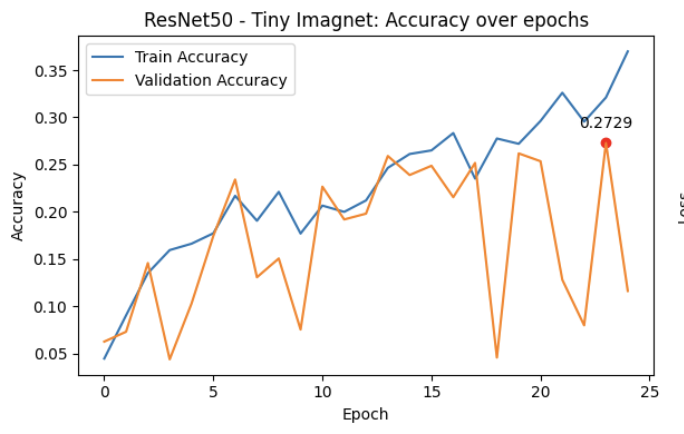
\includegraphics[width=0.8\linewidth]{resnet50_tiny_imagenet_training_graph.png}
    \caption{Training graph of ResNet-50 on Tiny ImageNet showing spikiness in validation performance.}
    \label{fig:spikygraph}
\end{figure}

\section{State of the Art in Computer Vision}

Recent advancements in the field of computer vision, particularly concerning image classification, have presented novel methodologies and optimizations that have pushed the boundaries of model accuracy and efficiency. 

The \textbf{Lion} optimizer, for example, has demonstrated remarkable success, achieving 91.1\% fine-tuning accuracy on ImageNet. Notably, Lion is engineered to amalgamate the advantages of both Adam and SGD optimizers, balancing rapid convergence with stable training \cite{chen2023symbolic}.

Another noteworthy development is the \textbf{Contrastive Captioner (CoCa)} model, which achieved a noteworthy 91.0\% top-1 accuracy on ImageNet with a fine-tuned encoder. CoCa incorporates a hybrid pretraining strategy, integrating contrastive loss and captioning loss, offering the model capabilities of both contrastive approaches like CLIP and generative methodologies like SimVLM \cite{yu2022coca}. 

Lastly, the concept of \textbf{Model Soups} offers a novel perspective on model optimization. Instead of discarding models from hyperparameter tuning sessions, it proposes averaging the weights of multiple fine-tuned models, which has empirically improved accuracy without increasing inference time. This methodology has seen particular success when fine-tuning large pre-trained models like CLIP, ALIGN, and a ViT-G pre-trained on JFT \cite{pmlr-v162-wortsman22a}.

\section{Conclusion and Future Work}

This study offered an in-depth exploration into the realm of image classification using neural networks, investigating the performance of custom CNN architectures and comparing them against widely-recognized networks like VGG16 and ResNet50 on popular datasets. The experimental results, observations, and insights derived from this exploration can serve as a foundation for further research and optimization in the domain of image classification using deep learning models.

In future work, exploring additional architectures such as EfficientNet, exploring additional regularization techniques for handling complex datasets like Tiny ImageNet, and investigating further into the phenomenon of "Grokking" may offer further insights and improvements in the field of image classification using neural networks.

\section*{Acknowledgments}
I'd like to thank ChatGPT \cite{ChatGPT2023} for assistance with formatting, editing, and LaTeX support throughout this assignment.

\bibliography{aaai23}

\end{document}
